Since $\vec{x_1}$ and $\vec{x_2}$ lie on the circle,
\begin{align}
       \vec{x_1}^\top\vec{x_1}+2\myvec{g&f}\vec{x_1}+c=0\\
       \vec{x_2}^\top\vec{x_2}+2\myvec{g&f}\vec{x_2}+c=0
\end{align}
Subtracting the two, we get,
\begin{align}
    \vec{x_2}^\top\vec{x_2}-\vec{x_1}^\top\vec{x_1}=-2\myvec{g&f}(\vec{x_2}-\vec{x_1}) \label{rams/4/2/21/a}
\end{align}
The midpoint of the chord $\vec{x_1x_2}$ is 
\begin{align}
    \vec{M}=\dfrac{\vec{x_1}+\vec{x_2}}{2}
\end{align}
Since perpendicular bisector of $\vec{x_1x_2}$ is perpendicular to $\vec{x_1x_2}$ and passes through $\vec{M}$, any general point $\vec{P}$ on the perpendicular bisector can be given using the relation
\begin{align}
    &\left(\vec{x_2}-\vec{x_1}\right)^\top\left(\vec{P}-\vec{M}\right)=0\\
    \implies &\left(\vec{x_2}-\vec{x_1}\right)^\top\vec{P}-\left(\vec{x_2}^\top-\vec{x_1}^\top\right)\left(\dfrac{\vec{x_1}+\vec{x_2}}{2}\right)=0\\
    \implies &\left(\vec{x_2}-\vec{x_1}\right)^\top\vec{P}=\dfrac{\vec{x_2}^\top\vec{x_2}-\vec{x_1}^\top\vec{x_1}+\vec{x_2}^\top\vec{x_1}-\vec{x_1}^\top\vec{x_2}}{2}
\end{align}
Since $\vec{x_1}^\top\vec{x_2}=\vec{x_2}^\top\vec{x_1}$, the equation reduces to
\begin{align}
    2\left(\vec{x_2}-\vec{x_1}\right)^\top\vec{P}=\vec{x_2}^\top\vec{x_2}-\vec{x_1}^\top\vec{x_1}
\end{align}
Using \eqref{rams/4/2/21/a}, we get
\begin{align}
    2\left(\vec{x_2}-\vec{x_1}\right)^\top\vec{P}&=-2\myvec{g&f}(\vec{x_2}-\vec{x_1})\\
    \implies \left(\vec{x_2}-\vec{x_1}\right)^\top\vec{P}&=\left(\vec{x_2}-\vec{x_1}\right)^\top\myvec{-g\\-f}
\end{align}
Since the centre of the circle is $\vec{C}=\myvec{-g\\-f}$, we can clearly see that $\vec{P}=\vec{C}$ satisfies the equation of perpendicular bisector.\\

Hence, the perpendicular bisector of any chord of a circle passes through the centre of the circle.\\

For example, consider the circle
\begin{align}
    \vec{x}^\top\vec{x}+2\myvec{-4&-5}\vec{x}+5=0
\end{align}
and let $\vec{x_1}=\myvec{0\\5-2\sqrt{5}}$ and $\vec{x_2}=\myvec{-2\\5}$.
We can clearly see in Fig.     \ref{rams/4/2/21/fig} that the perpendicular bisector the chord $\vec{x_1x_2}$ passes through the centre of the circle.

\begin{figure}[h!]
    \centering
    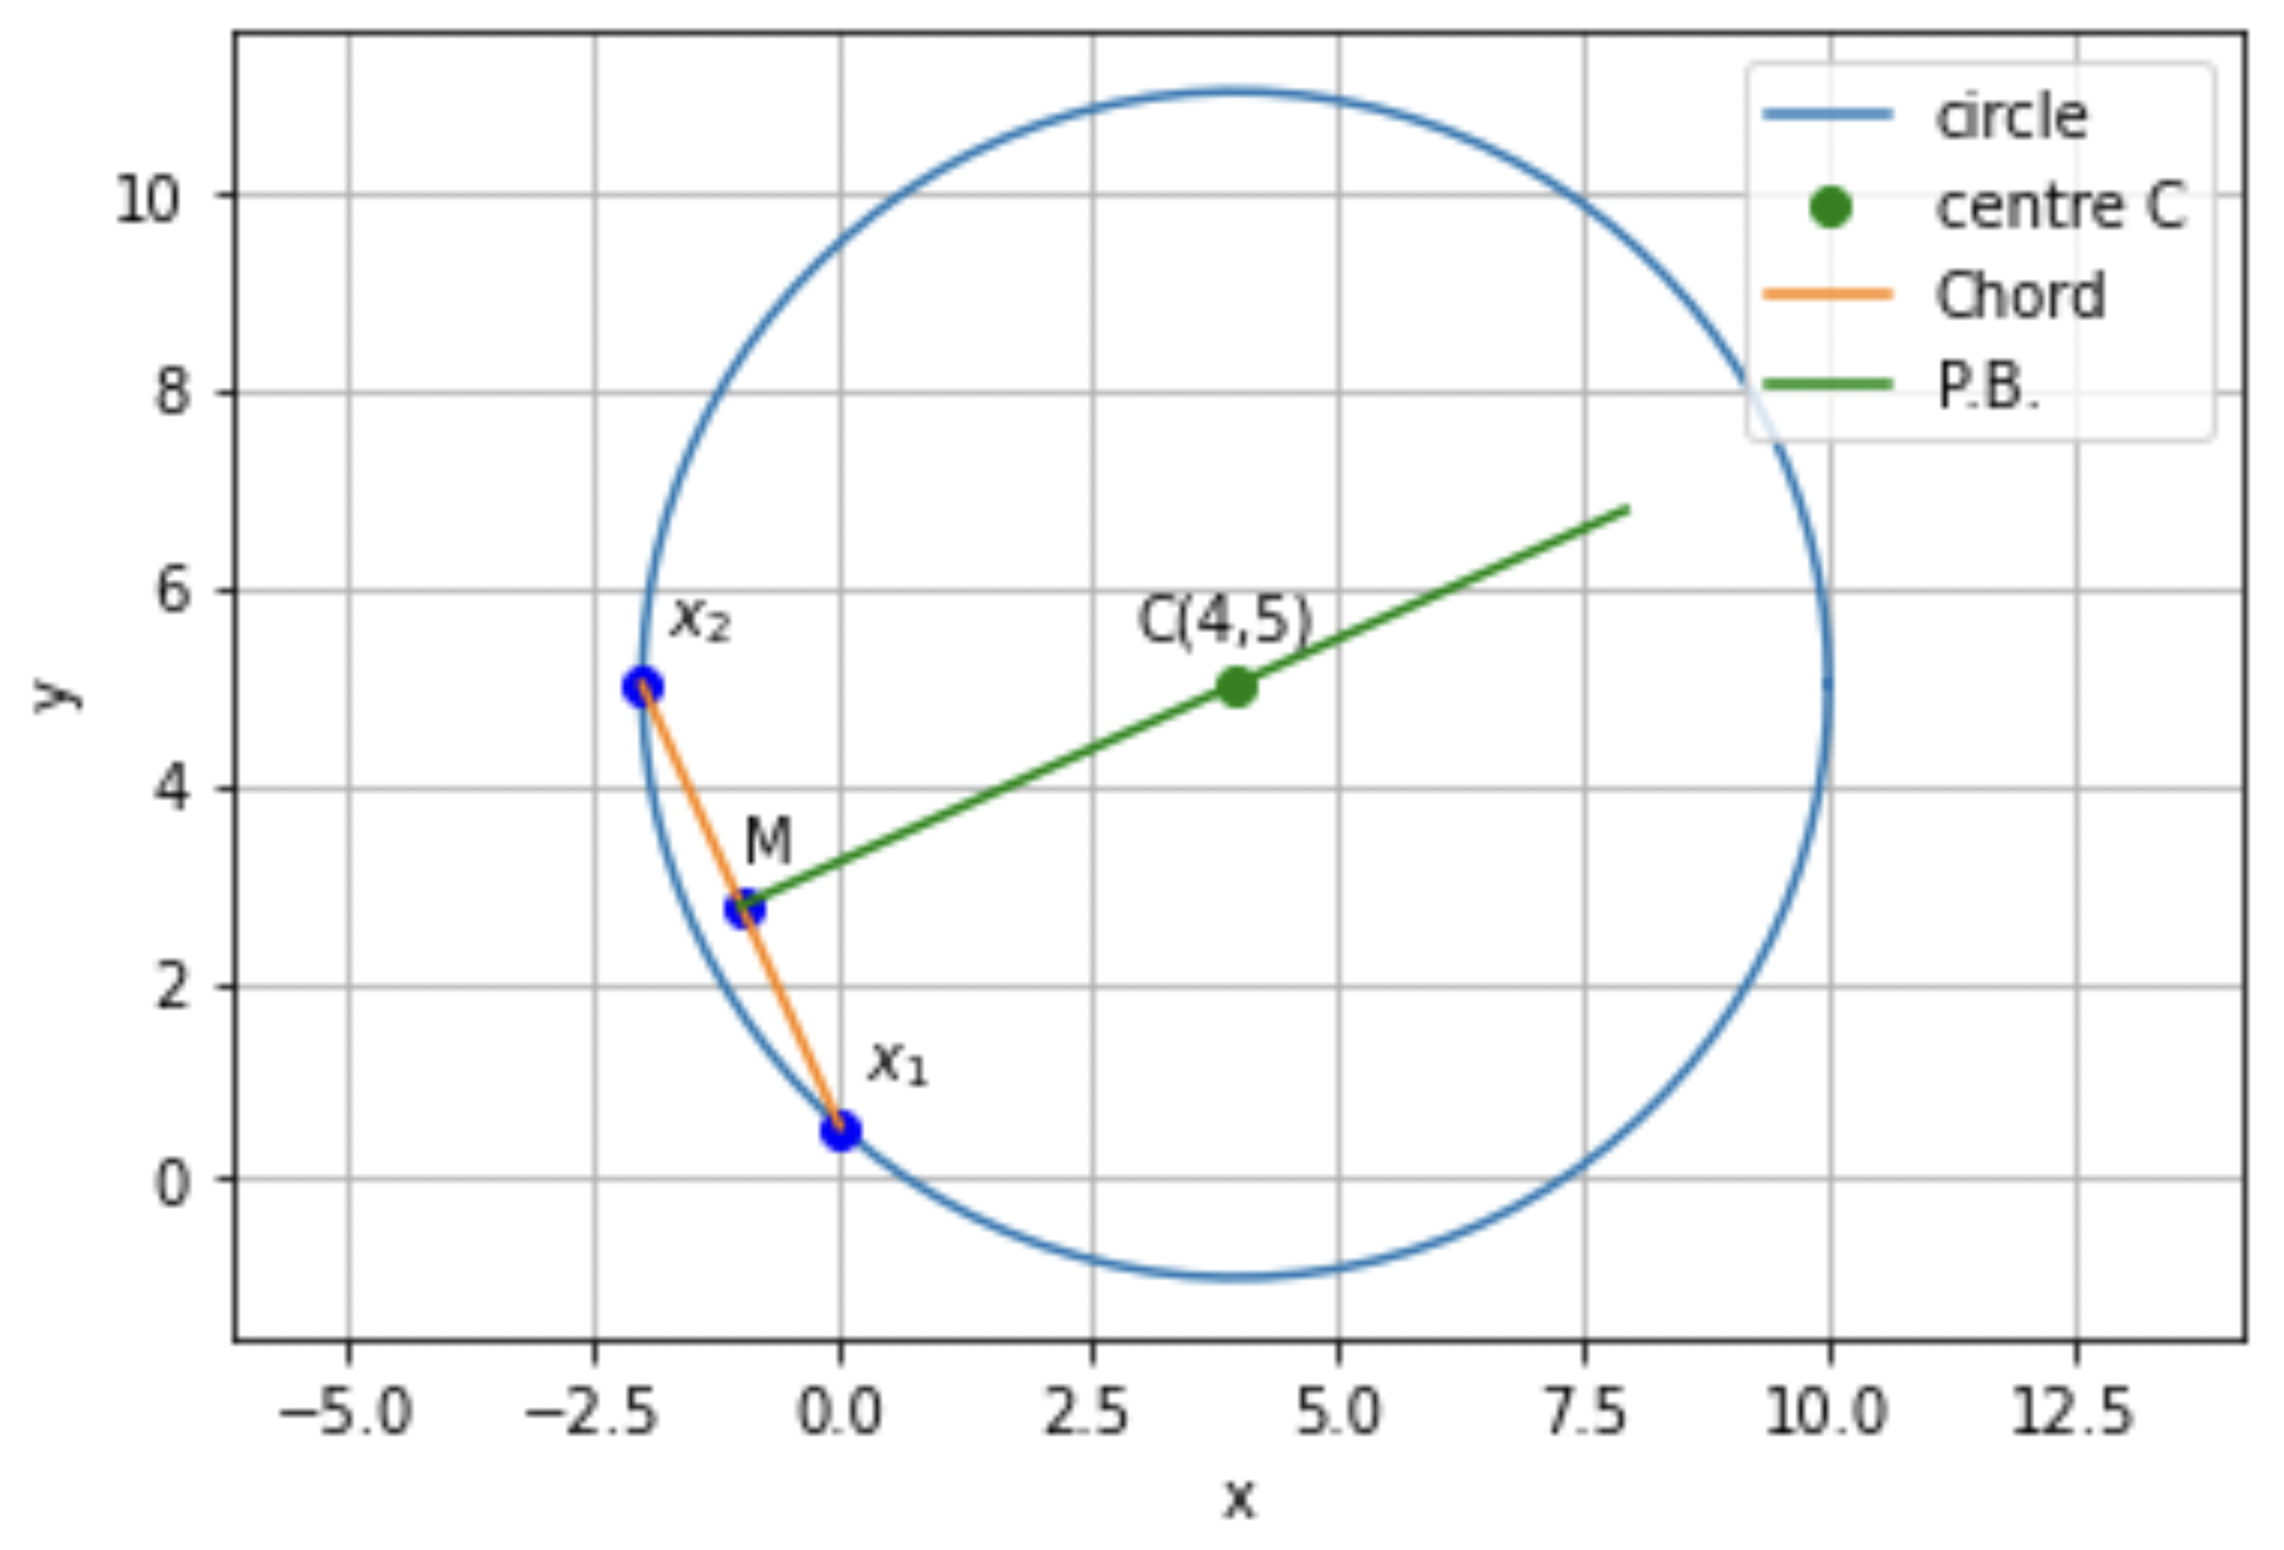
\includegraphics[width=\columnwidth]{solutions/4/2/21/figures/example_figure.png}
    \caption{Example figure}
    \label{rams/4/2/21/fig}
\end{figure}


